\section{Introduction} % (fold)
\label{sec:Introduction}

\subsection{Problématique et contexte} % (fold)
\label{sub:prob_contexte}

Le club étudiant Chinook\footnote{\url{http://chinookets.com}} de l'ÉTS est un regroupement d'étudiants qui analysent, concoivent et construisent un véhicule propulsé par une éolienne [figure \ref{fig:chinookHall}]. Le véhicule participe, chaque année, depuis deux années à une compétition de véhicules du même type et participe à des courses contre la montre. Le véhicule est ensuite évalué selon sa performance en fonction de sa vitesse par rapport à la vitesse du vent.

La compétition vise à ammener les étudiants a développer de nouvelles technologies pour les éoliennes, plus précisément pour des éoliennes de petites dimensions. Afin de rendre la compétition intéressante, elle sont utilisées en tant que moteur d'un véhicule de petite dimension. Un tel véhicule ne serait pas viable mais une telle technologie pourrait facilement être adapté sur d'autre médiums tels que les éoliennes sur des navires ou pour des batiments.

\begin{figure}[H]
  \centering
  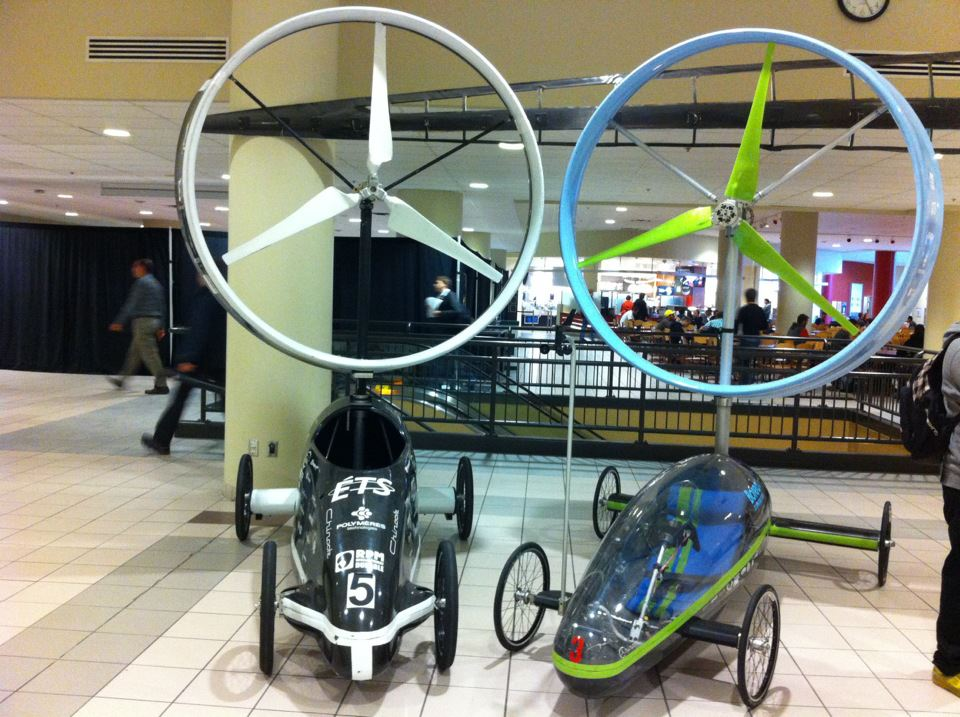
\includegraphics[width=0.5\textwidth]{images/chinook_1_2.jpg}
  \caption[Chinook 1 et 2]{Le Chinook 1 et le Chinook 2 en exposition dans le Hall A de l'ÉTS}
  \label{fig:chinookHall}
\end{figure}

Pour améliorer le véhicule, permettre de à l'équipe de bien performer et rester compétitif l'équipe installe un système électro-mécanique de contrôle de l'angle d'attaque des pâles. La transmission du véhicule sera aussi modifiée afin de pouvoir être asservi électroniquement.

Afin de pouvoir contrôller ces systèmes électroniques, des modèles de contrôle et d'optimisation de la puissance de l'éolienne doivent être créés. Les modèles disponibles sur les éoliennes statique peuvent s'appliquer pour une éolienne en mouvement mais doivent être modifiés afin de prendre en compte plusieurs facteurs.

%--------------------------------------------------------
%--TODO: ------------------------------------------------
... réciter les papers ici
%--------------------------------------------------------
%--------------------------------------------------------

% subsection Problématique et contexte (end)
\subsection{Objectifs} % (fold)
\label{sub:Objectifs}

% subsection Objectifs du projet (end)

% section Introduction (end)
